\documentclass[paper=a4, fontsize=11pt]{scrartcl}
\usepackage[T1]{fontenc}
\usepackage{fourier}

\usepackage[english]{babel}															% English language/hyphenation
\usepackage[protrusion=true,expansion=true]{microtype}	
\usepackage{amsmath,amsfonts,amsthm} % Math packages
\usepackage[pdftex]{graphicx}	
\usepackage{url}
\usepackage{tikz}

%%% Custom sectioning
\usepackage{sectsty}
\allsectionsfont{\centering \normalfont\scshape}


%%% Custom headers/footers (fancyhdr package)
\usepackage{fancyhdr}
\pagestyle{fancyplain}
\fancyhead{}

% No page header
\fancyfoot[L]{}											% Empty 
\fancyfoot[C]{}											% Empty
\fancyfoot[R]{\thepage}									% Pagenumbering
\renewcommand{\headrulewidth}{0pt}			% Remove header underlines
\renewcommand{\footrulewidth}{0pt}				% Remove footer underlines
\setlength{\headheight}{13.6pt}


%%% Equation and float numbering
\numberwithin{equation}{section}		% Equationnumbering: section.eq#
\numberwithin{figure}{section}			% Figurenumbering: section.fig#
\numberwithin{table}{section}				% Tablenumbering: section.tab#


%%% Maketitle metadata
\newcommand{\horrule}[1]{\rule{\linewidth}{#1}} 	% Horizontal rule

\title{
		%\vspace{-1in} 	
		\usefont{OT1}{bch}{b}{n}
		\normalfont \normalsize \textsc{Joy of Computer Science} \\ [25pt]
		\horrule{0.5pt} \\[0.4cm]
		\huge Geometric Algorithms -- The Convex Hull Problem in 2 \& 3 Dimensions \\
		\horrule{2pt} \\[0.5cm]
}
\author{
		\normalfont 								\normalsize
        M. Usaid Rehman\\[-3pt]		\normalsize
        \texttt{mr04302}
        \and 
        \normalfont 								\normalsize
        Syed Anus Ali\\[-3pt]		\normalsize
        \texttt{aa04928}
        \and 
        \normalfont 								\normalsize
        Faraz Ozair\\[-3pt]		\normalsize
        \texttt{mo05005}
}
\date{}


%%% Begin document
\begin{document}
\maketitle

\section{Introduction to Computational Geometry}
\subsection{Overview}
 
\subsection{History of its applications}
Geometry has been central to mathematics since the time of the ancient Greeks and ancient Egyptians. Euclid, who was a Greek mathematician, had a profound influence on the study of geometry. Introduction of Coordinates permitted an increase in computational power which later on was used in the study of geometry as geometry has different dimensions and for each of those processing power used was much higher than previous ones, the most common ones were in 2D and 3D although 2D did not require much processing but 3D had to have a lot of processing power.\\
\\
The term "Computational Geometry" was coined first by 
Marvin Minsky in his famous book called "Perceptrons" in 1969. This book is about a parallel computer which is called the "Perceptron" which contains a number of readersthat scan a field independently and simultaneously,  and it makes decisions by linearly combining the local and partial data gathered, weighing the evidence, and deciding if events fit a given “pattern,” abstract or geometric. This book talks about this machine in 3 ways firstly being "algebraic" the general property of linear predicate families which apply to all "Perceptrons". The second part focuses more on geometric patterns and theorems and the third part talks about perceptrons as practical devices. \\
\\
There are multiple applications in this discipline like the Euclidean travelling salesperson, minimum spanning tree and linear programming etc. 
\section{Geometric Preliminaries}
\subsection{Definitions \& Notation}
There are some key components in computational geometry that we need to understand before we move on to solving a problem such as the Convex Hull which is both complex and at the same time interesting. \\
\\
The main objects considered when we talk about computational geometry are sets of points in Euclidean Space. \\
Sets of points are finite or we could say that they are at least finitely specifiable.
By $E^d$, we denote the $d$-\textit{dimensional Euclidean space}. and E is the Euclidean space. A $d$-tuple $(x_1,\dots, x_d)$ denotes a point of $E^d$ where $x_i \in \mathbb{R}$.A \emph{polygon} in $E^2$ is defined by a finite set of line segments where each extreme point is shared by exactly two segments called \textit{edges}.
A \textit{polyhedron} in $E^3$ is defined by a finite set of plane polygons such that every edge of a polygon is shared by only one other polygon.

\section{The Convex Hull Problem}
\subsection{Introduction}
A \emph{convex set} is a subset of Euclidean space where given any two points in the set,  the set contains the whole line segment joining them. A  \emph{convex hull} of a shape is the smallest convex set containing the shape.
The convex hull can also be defined as the intersection of all convex sets of a given subset of Euclidean space.
Computing the \emph{convex hull} is a problem in computational geometry. 

    \begin{figure} [H]
            \centering
            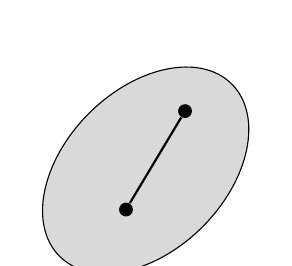
\begin{tikzpicture}
            \draw[rotate=-45,fill=gray!30] (0,0) ellipse (29pt and 44pt);
            \node[circle, fill=black,inner sep=0pt,minimum size=5pt] (A) at (0.5,0.75) {};
            \node[circle, fill=black,inner sep=0pt,minimum size=5pt] (B) at (-0.25,-0.5) {};
            \draw[thick] (A) -- (B) {};
            \end{tikzpicture}
            \caption{A convex set}
            \label{convex}
    \end{figure}
\subsection{Definition}

\section{Convex Hull Algorithms & Complexity}
\subsection{Lower Bound & Output Sensitivity}



\subsection{Algorithms}


%%% End document
\end{document}